% =============================================================================
% paper_v1.tex - ICU-Sepsis OOD-action study (NeurIPS 2026 format, DOUBLE-BLIND)
%
% v1 EXECUTOR FILL-IN, 2026-05-23. Derived from main.tex; Method + Experiments
% reused, and Abstract / Introduction / Related Work / Discussion / Conclusion
% prose written out. Blueprints: core_docs/paper_spec.md (read the top "v1
% decisions" block, then 0.0/0.3/per-section), core_docs/spec.md (format).
%
% TEAMMATE RESULTS: cross-algorithm + AA-MBRL numbers in Table 2 are the teammate's
% saved policies (committed in her repo) re-evaluated EXACTLY against the true dynamics
% via scripts/eval_teammate_policies.py (results/teammate_exact_eval/summary.json), so
% every trained value is <= V* (no rollout exceedance). No provisional numbers remain.
%
% TO COMPILE (Overleaf): drop neurips_2026.sty into the project. Anonymous
% submission mode (do NOT pass [final]) auto-prints "Anonymous Author(s)" and
% enables line numbers. The six PNGs live in submission/figures/ (graphicspath
% below also looks in ./figures/).
% ANONYMITY: no names / affiliations / real repo URLs anywhere.
% =============================================================================
\documentclass{article}

\usepackage{neurips_2026}            % submission mode = anonymous + line numbers
\usepackage[utf8]{inputenc}
\usepackage[T1]{fontenc}
\usepackage{hyperref}
\usepackage{url}
\usepackage{booktabs}
\usepackage{amsfonts}
\usepackage{amsmath}
\usepackage{amssymb}
\usepackage{graphicx}
\usepackage{microtype}
\usepackage{xcolor}
\usepackage{enumitem}                % for enumerate [leftmargin=...] options

% Look for figures in ./figures/ first, then in ../submission/figures/ where the
% six PNGs currently live, so the file compiles without moving assets.
\graphicspath{{figures/}{../submission/figures/}}

\newcommand{\Adm}{\mathcal{A}}
\newcommand{\dist}{\mathrm{dist}\text{-}V^\star}
\newcommand{\todo}[1]{\textcolor{red}{[TODO: #1]}}

\title{When Mean Imputation Hides Unsupported Actions:\\
Diagnosing and Repairing an Out-of-Distribution Action\\
Failure Mode in the ICU-Sepsis Benchmark}

\author{%
  Anonymous Author(s)\\
  Affiliation\\
  \texttt{email}\\
}

\begin{document}
\maketitle

\begin{abstract}
ICU-Sepsis's known dynamics let us measure the cost of out-of-distribution (OOD)
action handling exactly against the true optimal value $V^\star$, rather than
through the noisy off-policy estimation that real-data medical reinforcement
learning (RL) must otherwise rely on. ICU-Sepsis, a tabular MDP distilled from
MIMIC-III, ships a default \texttt{mean} strategy that sets the transition of
every inadmissible (data-unsupported) action to the \emph{average} of the
admissible actions in that state, and argues this is benign because it is
``equivalent to choosing a random admissible action.'' We show this design
carries a measurable cost that the benchmark's headline metric (survival rate)
hides: under the default, vanilla Q-learning deploys unsupported actions in
$\sim$87\% of states and converges to a policy value ($J{=}0.785$) no better than
the Random (0.780) and clinician (0.782) baselines, far from the optimum
($J^\star{=}0.875$). Evaluating every policy \emph{exactly} against $V^\star$, a
component ablation localizes the failure to \emph{behavior-level} sampling:
\emph{in our ablation}, restricting behavior to supported actions is necessary
and sufficient, while masking only the Bellman target or the deployed policy is
not (deployment masking leaves an exact, ground-truth $Q$-value leakage of
$+0.46$), and the leakage diagnostic explains \emph{why}. We then compare a
spectrum of support-aware remedies---support penalties, CQL-style conservatism,
admissibility masking, and a model-based endpoint---across Sarsa/Q/DQN/PPO and in
a finite-data offline empirical-MDP regime, where naive mean-imputation
overestimates its own value ($+0.21$) and stagnates while pessimism and masking
stay calibrated and improve with data. Our results are benchmark-internal and are
not clinical recommendations; what transfers is the phenomenon and a reusable
exact-$V^\star$ auditing protocol, and inadmissible-action handling should be
reported, not left to a hidden default.
\end{abstract}

% =============================================================================
\section{Introduction}
\label{sec:intro}
Three observations about ICU-Sepsis \citep{choudhary2024icusepsis}, a tabular
sepsis-treatment MDP distilled from real ICU records, motivate this paper.
\textbf{First}, a default data-imputation choice that the benchmark
\emph{explicitly} describes as harmless---``equivalent to choosing a random
admissible action''---leaves vanilla Q-learning stuck at the random baseline
($J{=}0.785$ vs.\ Random $0.780$). \textbf{Second}, the obvious fix of masking
unsupported actions \emph{at deployment} is not enough: it drives the deployed
unsupported-action rate to zero yet leaves the learned $Q$-table corrupted, with
an exact $Q$-value leakage unchanged at $+0.46$. \textbf{Third}, in a finite-data
offline regime, \emph{more} data makes the naive agent overestimate its own value
\emph{more}, not less ($+0.21$ and stagnating), contrary to the intuition that
more data should be more accurate. These tensions are the subject of this paper.

\paragraph{From a benchmark question to a measurement instrument.}
Handling actions with insufficient data support is a central, well-recognized
challenge in offline RL, whose typical consequence is value overestimation
\citep{fujimoto2019bcq,kumar2020cql}; on real medical data, however, it can only
be probed through off-policy estimators that are noisy and biased
\citep{gottesman2019guidelines,gottesman2018evaluating}. ICU-Sepsis is a rare
combination---distilled from real MIMIC-III trajectories yet shipping its full
dynamics---so we can evaluate any policy \emph{exactly} against the true optimal
value $V^\star$, sidestepping off-policy estimation entirely. We use this not as a
leaderboard but as a clean ruler for the OOD/unsupported-action pathology: a
real-distilled environment with ground-truth value and no need for OPE. Concretely,
this lets us turn the benchmark's own claim of benignness into a testable one and
show it does not hold: the default mean-imputation has a cost that survival rate hides.

\paragraph{Reframing and the central finding.}
We frame the benchmark's inadmissible actions as OOD / low-support actions, and
treat its known dynamics as a \emph{measurement instrument} (exact $V^\star$),
not an optimization target. With this instrument, our central finding is that the
decisive remedy is \emph{not} to mask unsupported actions at deployment---the
obvious move, which still leaves the $Q$-table corrupted---but to keep them out of
the \emph{behavior} that is sampled and bootstrapped during training:
\emph{in our component ablation}, this behavior-level restriction is both
necessary \emph{and} sufficient, and an exact, ground-truth $Q$-value-leakage
diagnostic explains the mechanism. Generality across learning algorithms, a
model-based remedy endpoint, and a finite-data offline regime serve as
\emph{supporting evidence} that the phenomenon and its remedy hold broadly, not as
separate claims. A representative result: under the default, an agent deploys
unsupported actions in $\sim$87\% of states yet scores at the random/clinician
level ($0.785$ vs.\ $0.780/0.782$), and behavior-level admissibility control
recovers $\dist$ from $0.090$ to $0.069$.

\paragraph{Structure the benchmark ships but baselines discard.}
Beyond the mean-imputation default, ICU-Sepsis carries per-state structure that
standard agents drop during training: which actions have data support
(admissibility), an empirical transition model, a severity score, and a clinician
behavior policy. Our main line uses admissibility (P1) and the empirical model
(P2); severity-based shaping and the clinician prior are supplementary. This
framing motivates the remedy spectrum: putting the discarded structure back is
enough to remove the pathology and close the artificial gap.

\paragraph{Contributions.}
\begin{enumerate}[leftmargin=2em,itemsep=2pt,topsep=2pt]
  \item \textbf{A benign-design claim with a hidden, exactly-measurable cost.}
  ICU-Sepsis explicitly argues its default mean-imputation is harmless
  (\emph{``equivalent to choosing a random admissible action''}); using the
  benchmark's known dynamics to evaluate against the true $V^\star$, we show it
  carries a measurable cost that survival rate hides---vanilla model-free agents
  deploy unsupported actions in $\sim$87\% of states and converge to $J{=}0.785$,
  no better than Random (0.780) / clinician (0.782) (\S\ref{sec:failure}).
  \item \textbf{Mechanism, not merely a fix (our central result).} A component
  ablation plus an exact $Q$-value-leakage diagnostic localize the failure to
  \emph{behavior-level} sampling: \emph{in our ablation}, restricting behavior to
  supported actions matches the full mask and is the only component that clears the
  $Q$-value leakage (necessary and sufficient to reach the full-mask result),
  whereas masking only the Bellman target or the deployed policy does not suffice
  (deployment-masking leaves leakage at $+0.46$)
  (\S\ref{sec:mechanism}).
  \item \textbf{Generality of the diagnosis and remedy, as supporting evidence.}
  The phenomenon and the support-aware remedy spectrum (support penalty $\to$ CQL
  conservatism $\to$ admissibility masking $\to$ model-based endpoint AA-MBRL)
  hold across Sarsa/Q/DQN/PPO and in a finite-data offline empirical-MDP regime,
  where naive imputation overestimates its own value ($+0.21$) and stagnates
  while pessimism and masking stay calibrated (\S\ref{sec:remedy}).
  \item \textbf{A reusable exact-$V^\star$ auditing protocol.} We package the
  study as an evaluation protocol for auditing OOD-action handling---three
  exactly-computable diagnostics (deployed-unsupported rate, $Q$-value leakage,
  value overestimation)---and release one-command scripts; ICU-Sepsis results
  should report inadmissible-action handling explicitly.
\end{enumerate}

% =============================================================================
\section{Related Work}
\label{sec:related}
\paragraph{Medical RL benchmarks.}
Sepsis treatment has been a recurring testbed for RL in healthcare
\citep{komorowski2018aiclinician,raghu2017continuous}, but learning from logged
clinical data is hampered by unknown dynamics and unreliable evaluation.
ICU-Sepsis \citep{choudhary2024icusepsis} and related curated benchmarks
\citep{mimic_sepsis_arxiv2510_24500} distill such data into reproducible MDPs.
Our work differs by treating such a benchmark as a \emph{measurement instrument}
for a specific pathology---using its exact $V^\star$ to audit how data-unsupported
actions are handled---rather than as a leaderboard to top.

\paragraph{Offline RL and OOD actions.}
The danger of bootstrapping from out-of-distribution actions, and the resulting
value overestimation, is the motivating problem for batch-constrained,
behavior-regularized, and conservative offline methods
\citep{fujimoto2019bcq,kumar2019bear,kumar2020cql}, with pessimism shown to be
provably and practically effective \citep{rashidinejad2021pessimism,jin2021pessimism}.
Our work differs by measuring this recognized pathology \emph{exactly} against
ground-truth $V^\star$ in an environment distilled from real data, isolating where
in the learning update the failure originates.

\paragraph{Invalid / forbidden action masking.}
Masking unavailable actions is standard in deep RL, both as an analysis target in
policy-gradient methods \citep{huang2021masking} and as a way to learn from
forbidden actions \citep{seurin2020forbidden}, and is available off-the-shelf as
maskable policies \citep{raffin2021sb3}. We
do not introduce masking; instead, a component ablation shows precisely \emph{where}
it must act---at the behavior level---and that masking only the target or only the
deployed policy is insufficient.

\paragraph{Tabular model-based RL.}
For small tabular MDPs, optimism- and posterior-sampling-based model-based methods
are known to be near-optimal \citep{auer2008ucrl,osband2013psrl}. We
\emph{acknowledge} that a $716$-state model-based agent reaching $V^\star$ is
expected, not a feat; we therefore frame our model-based remedy as the endpoint of
a spectrum that demonstrates the gap is an artifact of mean-imputation, and our
contribution is the diagnosis and mechanism, not a regret or optimality result.

\paragraph{Reward shaping and behavior-constrained learning.}
Potential-based reward shaping leaves the optimal policy invariant
\citep{ng1999reward}, which justifies our supplementary severity-based shaping;
constraining a learner toward a behavior policy is likewise a standard offline-RL
device \citep{wu2019behavior,nair2020awac}.
Our work differs by using these only as supplementary points on the remedy
spectrum, with admissibility---not shaping---as the load-bearing structure.

\paragraph{Evaluation pitfalls in healthcare RL.}
Off-policy evaluation in observational health settings is noisy and easily
misleading \citep{gottesman2019guidelines,gottesman2018evaluating}. Our work
differs by sidestepping OPE entirely: exact $V^\star$ makes selection rates,
value gaps, and overestimation measurable in a way real cohorts do not allow.

% =============================================================================
\section{Background: ICU-Sepsis and Mean Imputation}
\label{sec:background}
ICU-Sepsis \citep{choudhary2024icusepsis} is a tabular MDP with $|\mathcal{S}|{=}716$
states (713 patient states plus death, survival, $s_\infty$) and $|\mathcal{A}|{=}25$
actions (5 fluid $\times$ 5 vasopressor levels). The reward is a survival indicator
(${+}1$ on transition into the survival state, $0$ otherwise) and $\gamma{=}1$, so
episodes are short and the undiscounted return equals the survival probability;
consequently $V^\star(s)$ is exactly the maximum achievable survival probability
from $s$. Because the full transition model is shipped with the benchmark, we
compute $V^\star$ and the exact value $V^\pi$ of any policy by value iteration,
avoiding off-policy estimation entirely.

\paragraph{Admissibility and the \texttt{mean} strategy.}
Each state has an \emph{admissible} action set $\Adm(s)$: actions taken at least
$\tau{=}20$ times in the source cohort, so their transition estimates are reliable.
The remaining actions are \emph{inadmissible} (data-unsupported); admissible sets
are small (median 4, mean 3.2, of 25). For an inadmissible action $a\notin\Adm(s)$,
the benchmark's default \texttt{mean} strategy defines the transition as the
unweighted average over admissible actions:
\begin{equation}
\label{eq:mean}
P(s'\mid s,a) \;=\; \frac{1}{|\Adm(s)|}\sum_{a'\in\Adm(s)} \zeta(s,a',s'),
\qquad a\notin\Adm(s),
\end{equation}
where $\zeta$ is the empirical admissible-action transition. We verified
Eq.~\eqref{eq:mean} holds exactly in the shipped dynamics (every inadmissible row
equals the admissible mean to $7\times10^{-16}$). The benchmark motivates this as
``equivalent to choosing a random admissible action'' \citep{choudhary2024icusepsis};
\S\ref{sec:failure} shows this equivalence is precisely where the cost arises.

% =============================================================================
\section{Method: Support-Aware Tabular RL}
\label{sec:method}
We frame inadmissible actions as \emph{out-of-distribution (OOD)} / low-support
actions, the central object of offline RL \citep{fujimoto2019bcq,kumar2020cql},
and study a spectrum of remedies that all share a tabular $Q:\mathcal{S}\times
\mathcal{A}\to\mathbb{R}$ update, isolating the effect of \emph{where} support is
enforced rather than of function approximation.

\paragraph{Remedy spectrum.}
(i) \emph{Vanilla} Q-learning over all 25 actions.
(ii) \emph{Support penalty}: $r'(s,a,s') = r - \lambda\,\mathbb{1}[a\notin\Adm(s)]$,
a learnable negative signal at the behavior/reward level, $\lambda\in\{0.01,\dots,1\}$.
(iii) \emph{CQL-style conservatism}: at each visited state, nudge $Q(s,\cdot)$ toward
the admissible support, $Q(s,\cdot)\!\mathrel{-}=\!\alpha\kappa\,(\mathrm{softmax}(Q(s,\cdot)) -
u_{\Adm(s)})$ with $u_{\Adm(s)}$ uniform on $\Adm(s)$ --- a value-level conservatism.
(iv) \emph{Admissibility masking}, decomposed into three independently-toggleable
components: \textbf{behavior} (restrict $\epsilon$-greedy selection to $\Adm(s)$),
\textbf{target} (restrict the Bellman backup $\max$ to $\Adm(s')$), and \textbf{policy}
(restrict the final greedy extraction to $\Adm(s)$). Hard masking enables all three.
(v) \emph{Admissibility-aware model-based RL (AA-MBRL)}, the model-based endpoint of
the spectrum: while interacting, we estimate an empirical model
$\hat P(s'\mid s,a){=}N(s,a,s')/N(s,a)$ (reward by running mean) and every
$K{=}1000$ episodes re-solve an \emph{admissibility-constrained} value iteration on
$\hat P$ restricted to $\Adm(s)$ (using $\gamma_{\mathrm{vi}}{=}0.999$ for
convergence since $\gamma{=}1$; $\epsilon$ annealed $0.5{\to}0.001$). We include
AA-MBRL not as a proposed algorithm but as the spectrum's right end: it shows that
even the most naive use of the benchmark's shipped model structure closes an
artificial gap.\footnote{AA-MBRL is implemented in the teammate's released code; we report its final
policy exactly evaluated against the true dynamics (\S\ref{sec:remedy}).}

\paragraph{Metrics (all exact unless noted).}
distance-to-$V^\star$, $\dist(\pi)=\mathbb{E}_{s\sim d_0}[V^\star(s)-V^\pi(s)]$;
deployed unsupported-action rate, the fraction of (non-terminal) states where the
greedy policy picks $a\notin\Adm(s)$; \emph{Q-value leakage},
$\frac{1}{|\mathcal{S}_{\mathrm{nt}}|}\sum_s\!\big[\max_{a\notin\Adm(s)}Q(s,a)-
\max_{a\in\Adm(s)}Q(s,a)\big]$, positive when unsupported actions are over-valued
(averaged over non-terminal states, each of which retains both admissible and
inadmissible actions; $Q$ lies on the $[0,1]$ survival-probability scale, so leakage
near $+0.5$ is about half the achievable range, with no further normalization);
value \emph{overestimation} (offline), the model's self-estimate minus the true
value; and agreement with the clinician policy.

% =============================================================================
\section{Experiments}
\label{sec:experiments}
\paragraph{Setup.} Unless stated otherwise, mechanism runs use 5 seeds,
$5{\times}10^4$ episodes, $\alpha{=}0.1$, $\gamma{=}1$, $\epsilon$ annealed
$1.0{\to}0.05$ over $10^4$ episodes. The cross-algorithm and model-based results
(Table~\ref{tab:merged}) use $5{\times}10^5$ episodes; \emph{each table states its
episode budget}, and the two budgets are bridged by the fact that vanilla
Q-learning stays at the baseline level at both ($J{=}0.785$ at $5{\times}10^4$;
$0.787$ exact at $5{\times}10^5$, Table~\ref{tab:merged}), so the failure is not
under-training. We report mean $\pm$ std (per-seed scatter in the
appendix); we do not rest conclusions on small survival differences but on
large-support diagnostics.

\paragraph{Baselines reproduce the benchmark (Table~\ref{tab:baselines}).}
Exact $d_0$-weighted values match the published Random/Expert/Optimal numbers,
confirming the ruler is calibrated; note also that survival values live in a narrow
$0.78$--$0.875$ band, motivating the more sensitive $\dist$.

\begin{table}[t]
\centering
\caption{Exact baseline reproduction ($d_0$-weighted policy value $=$ survival
rate). Exact value-iteration computations (budget-independent).}
\label{tab:baselines}
\begin{tabular}{lccc}
\toprule
 & Random & Clinician (Expert) & Optimal ($V^\star$) \\
\midrule
$J(\pi)$ & 0.780 & 0.782 & 0.875 \\
\bottomrule
\end{tabular}
\end{table}

\subsection{The hidden failure (Claim 1)}
\label{sec:failure}
Under the default \texttt{mean} strategy, vanilla Q-learning deploys inadmissible
actions in $\sim$87\% of states and reaches $J(\pi){=}0.785$ and
$\dist{=}0.090$ --- essentially the Random (0.780) / clinician (0.782) baselines.
Crucially, this is \emph{not} a mere labeling artifact: because an inadmissible
action behaves like a random admissible one (Eq.~\eqref{eq:mean}), selecting it
implements an average-over-admissible transition---competitive under bootstrapping
but unable to recover the best admissible action---which induces a measurable value
gap to $V^\star$. Survival rate hides this (the benchmark reports only
return/length/convergence); $\dist$ exposes it. Admissibility control recovers
$J{=}0.806$, $\dist{=}0.069$ (at $5{\times}10^4$; consistent with the exactly-evaluated $5{\times}10^5$ AA-Q policy, $J{=}0.801$/gap $0.074$, Table~\ref{tab:merged}). The failure is not specific to Q-learning or to a
small training budget: it persists across Sarsa/Q/DQN/PPO, and Q-learning still sits at the
baseline level ($J{=}0.787$ exact) at $5{\times}10^5$ episodes (Table~\ref{tab:merged}).

\subsection{Mechanism: where the failure lives (Claim 2)}
\label{sec:mechanism}
A component ablation (Table~\ref{tab:ablation}; Fig.~\ref{fig:ablation}) localizes
the failure to behavior-level sampling. \emph{In this ablation}, masking behavior
alone matches the full mask and is the only component that clears the $Q$-value
leakage---necessary and sufficient \emph{to reach the full-mask result}. The other
components help only marginally: masking only the target leaves $\sim$77\% deployed
unsupported, and masking only the deployed policy zeroes deployment but leaves the
$Q$-table corrupted (leakage unchanged at $+0.46$). The $Q$-value leakage flips from $+0.46$ (vanilla) to
$-0.80$ (behavior/full mask), showing unsupported actions become competitive only
because they are sampled and updated under mean-imputed dynamics. The sign of the
leakage is informative: a large \emph{negative} value (e.g.\ CQL $\kappa{=}1$:
$-2.95$) signals \emph{over}-suppression rather than a better policy, which is why
CQL ($\dist{=}0.080$) still trails hard masking ($0.069$) despite its strongly
negative leakage. This is the hero result of the paper; the breadth experiments
below support its generality.

\begin{table}[t]
\centering
\caption{Component ablation (5 seeds, $5{\times}10^4$ episodes). \emph{In this
ablation}, behavior masking is necessary and sufficient (matches the full mask).}
\label{tab:ablation}
\begin{tabular}{lcccl}
\toprule
Variant & $\dist\,\downarrow$ & Deploy unsupp. & Q-leakage & Reading \\
\midrule
vanilla            & 0.090 & 0.87 & $+0.46$ & unsupported over-valued \\
target-only        & 0.085 & 0.77 & $+0.07$ & backup alone insufficient \\
policy-only        & 0.083 & 0.00 & $+0.46$ & band-aid; $Q$ corrupted \\
CQL ($\kappa{=}1$) & 0.080 & 0.00 & $-2.95$ & best \emph{soft} remedy \\
\textbf{behavior-only} & \textbf{0.069} & 0.00 & $-0.80$ & necessary \& sufficient \\
full mask          & 0.069 & 0.00 & $-0.80$ & $=$ behavior-only \\
\bottomrule
\end{tabular}
\end{table}

% --- HERO FIGURE: highest priority; do not shrink or let Table 2 crowd it out. ---
\begin{figure}[t]\centering

\includegraphics[width=0.95\linewidth]{component_ablation.png}
\caption{\textbf{The mechanism (hero figure).} Component ablation (left) and
$Q$-value-leakage mechanism (right): masking \emph{behavior} is necessary and
sufficient (it matches the full mask), while masking only the target or only the
deployed policy does not remove the corruption; leakage flips from $+0.46$ to
$-0.80$ (5 seeds, $5{\times}10^4$ episodes).}
\label{fig:ablation}
\end{figure}

\subsection{Remedy spectrum, online and cross-algorithm (Claim 3a)}
\label{sec:remedy}
\paragraph{From soft to hard (single-algorithm, $5{\times}10^4$ episodes).}
Support penalties trace a support--value trade-off: larger $\lambda$ drives deployed
unsupported actions to $0$ (at $\lambda{=}1.0$) but $\dist$ plateaus ($\approx
0.085$) and is Pareto-dominated by hard masking ($0.069$); CQL-conservatism is the
best soft remedy ($0.080$) but still trails, with a $\kappa$ sweet spot ($\kappa{=}1$
helps, $\kappa{=}2$ over-suppresses to $0.089$) (Fig.~\ref{fig:spectrum}).

\begin{figure}[t]\centering
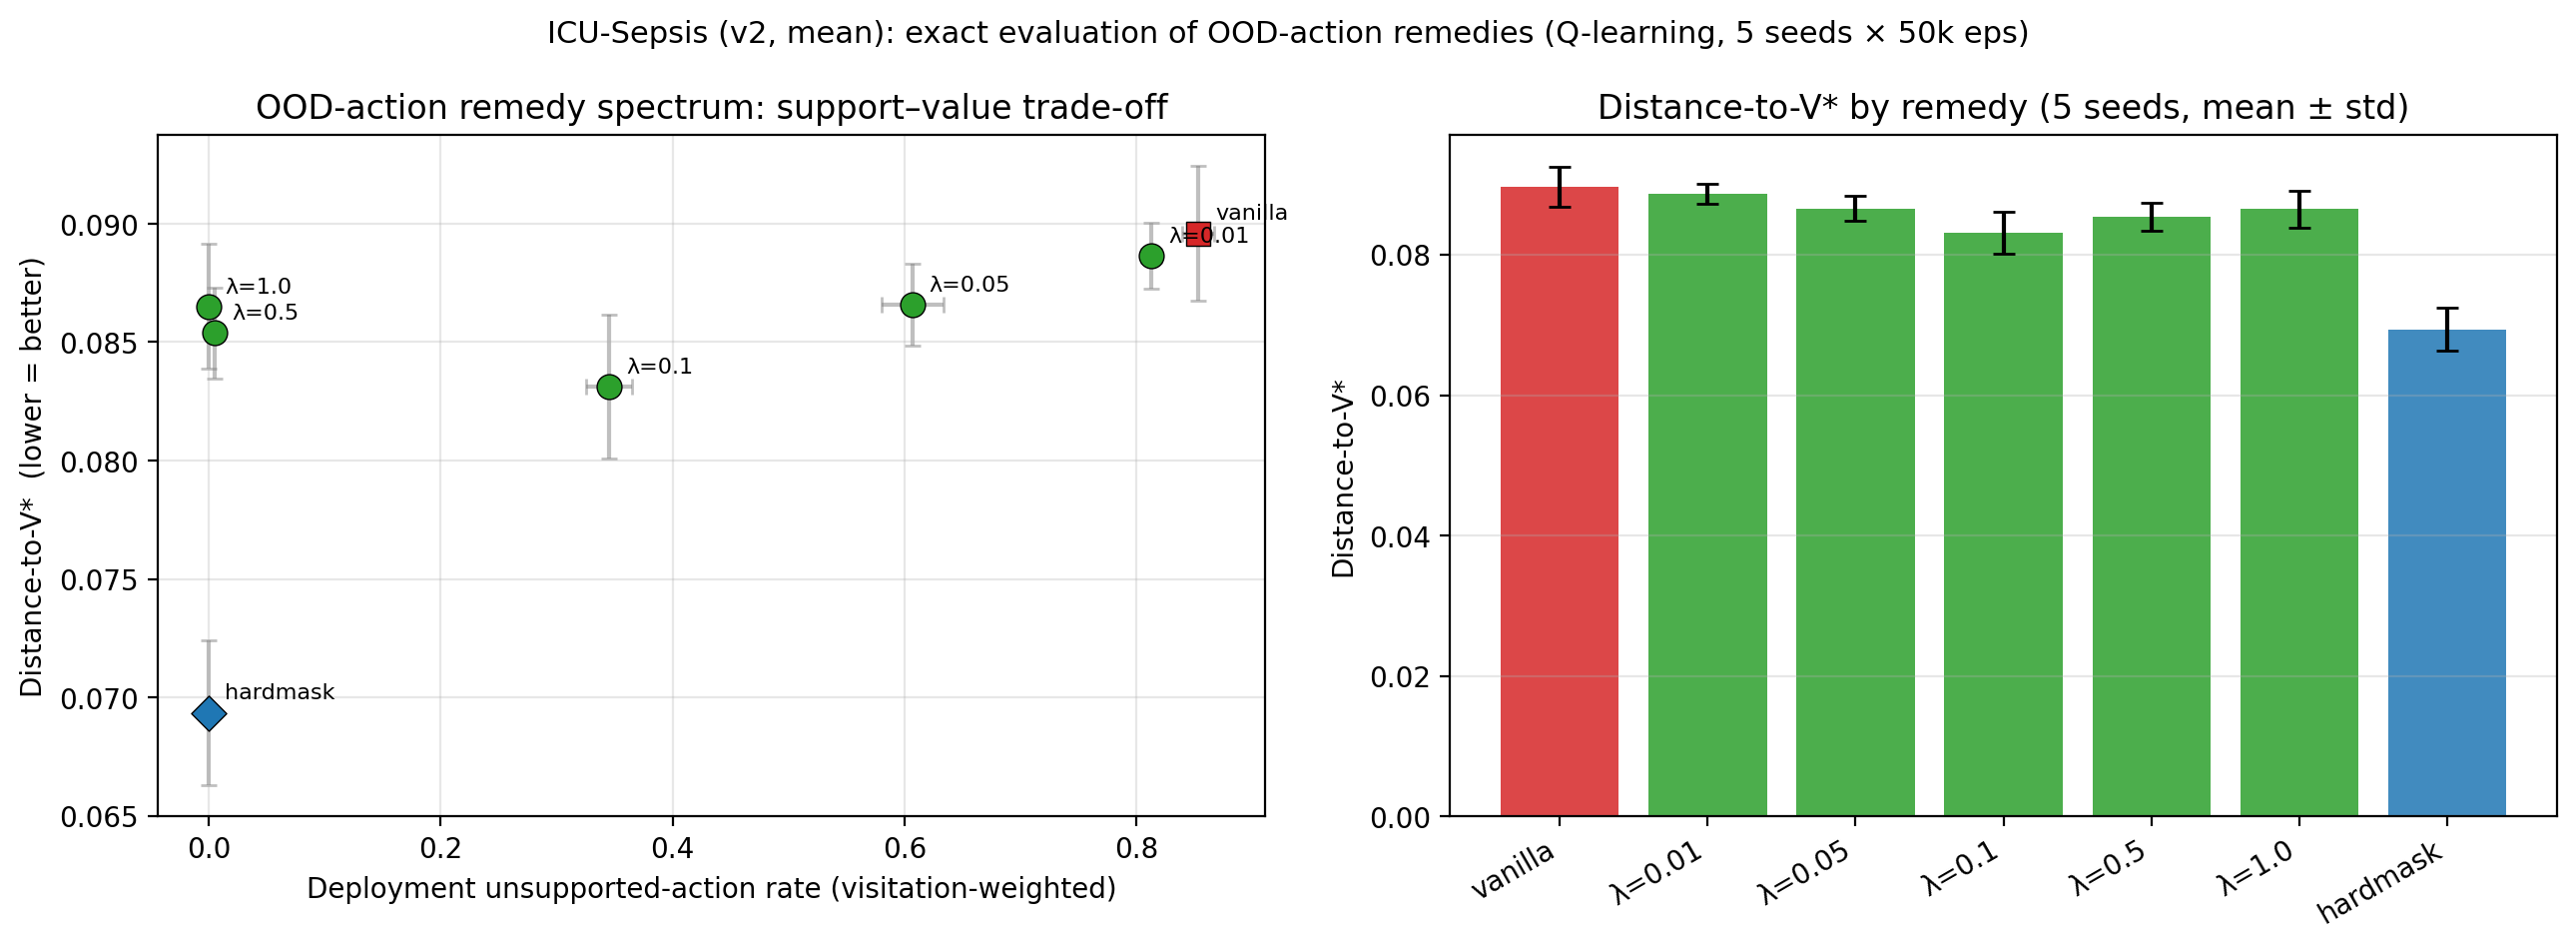
\includegraphics[width=0.85\linewidth]{penalty_tradeoff.png}
\caption{Remedy spectrum: the support--value trade-off; larger penalties remove
unsupported actions but plateau in $\dist$, and hard masking is Pareto-best
(5 seeds, $5{\times}10^4$ episodes).}
\label{fig:spectrum}
\end{figure}

\paragraph{Across algorithms and a model-based endpoint ($5{\times}10^5$ episodes).}
Table~\ref{tab:merged} reports the cross-algorithm picture, evaluated \emph{exactly}.
Admissibility masking improves every baseline---strictly positive on all four and
larger for the stronger baselines: exact $\dist$ gains of $+0.013$ (Sarsa), $+0.014$
(Q-learning), $+0.027$ (DQN), and $+0.027$ (PPO).\footnote{Policies are from the
teammate runs (committed in the released repo); we re-evaluate each exactly against
the true dynamics, so every trained value is $\le V^\star$. On the benchmark's rollout
metric the same masking effect is significant ($p\le0.013$) on the three stronger
baselines.} At the model-based endpoint, AA-MBRL reaches exact $J{=}0.874$ (gap
$0.001$). We read this not as ``winning'' but as confirmation that the gap is an
artifact of mean-imputation: even the most naive use of the shipped model structure
nearly closes it, and on a $716$-state tabular MDP a model-based agent reaching
$V^\star$ is expected \citep{auer2008ucrl,osband2013psrl}.

\begin{table}[t]
\centering
\caption{Cross-algorithm breadth, \emph{exactly} evaluated. Policies are from the
teammate runs ($5{\times}10^5$ episodes, 5 seeds, committed in the released repo); we
re-evaluate each saved policy exactly against the true dynamics ($V^\pi$ by value
iteration), on the same exact axis as the rest of the paper, so every trained value is
$\le V^\star$ --- unlike the benchmark's rollout metric, under which some near-optimal
cells spuriously exceed it. ``Deploy unsupp.'' is the deployed-state inadmissible-action
rate. The model-based endpoint AA-MBRL uses an online empirical model and is
\emph{not} a fair model-free comparison---supporting breadth showing the gap is an
artifact of ignoring support/model structure, not a headline result.}
\label{tab:merged}
\begin{tabular}{llccc}
\toprule
Group & Method & Exact $J(\pi)\uparrow$ & $\dist\downarrow$ & Deploy unsupp. \\
\midrule
Reference & Random            & 0.780 & 0.095 & --- \\
          & Clinician         & 0.782 & 0.093 & --- \\
          & Optimal $V^\star$ & 0.875 & 0.000 & --- \\
\midrule
No prior  & Sarsa       & 0.789 & 0.087 & 0.83 \\
          & Q-learning  & 0.787 & 0.088 & 0.85 \\
          & DQN         & 0.799 & 0.076 & 0.79 \\
          & PPO         & 0.842 & 0.033 & 0.58 \\
\midrule
$+$P1 mask & AA-Sarsa   & 0.802 & 0.073 & 0.00 \\
          & AA-Q        & 0.801 & 0.074 & 0.00 \\
          & AA-DQN      & 0.826 & 0.050 & 0.00 \\
          & AA-PPO      & 0.869 & 0.006 & 0.00 \\
\midrule
$+$P1$+$P2 & AA-MBRL    & 0.874 & 0.001 & 0.00 \\
\bottomrule
\end{tabular}
\end{table}

\subsection{Remedy spectrum, offline finite-data (Claim 3b)}
\label{sec:offline}
We collect $N$ transitions under the clinician behavior policy, build the
certainty-equivalent empirical model, and compare \emph{naive} (mean-impute unseen
actions), \emph{pessimistic} VI-LCB \citep{jin2021pessimism,rashidinejad2021pessimism},
and \emph{admissibility-masked} value iteration --- all evaluated exactly against
the true $V^\star$ (Fig.~\ref{fig:offline}). The support each method uses differs:
pessimism \emph{estimates} support from the $N$ samples (a count-based
lower-confidence bonus over observed actions), whereas masking uses the benchmark's
\emph{oracle} admissible set $\Adm(s)$; the masked cell therefore isolates the value
of known support labels, and pessimism the realistic estimate-from-data case. Naive overestimates its own value
($+0.21$ at $N{=}10^5$) and its realized policy \emph{stagnates}
($\dist\approx0.093$ regardless of $N$); pessimism is calibrated ($\approx0$) and
improves ($\to0.069$); masking removes unsupported actions and reaches $0.065$.
Exact $V^\star$ is what makes this overestimation pathology measurable --- normally
impossible in healthcare RL \citep{gottesman2019guidelines}.

\begin{figure}[t]\centering
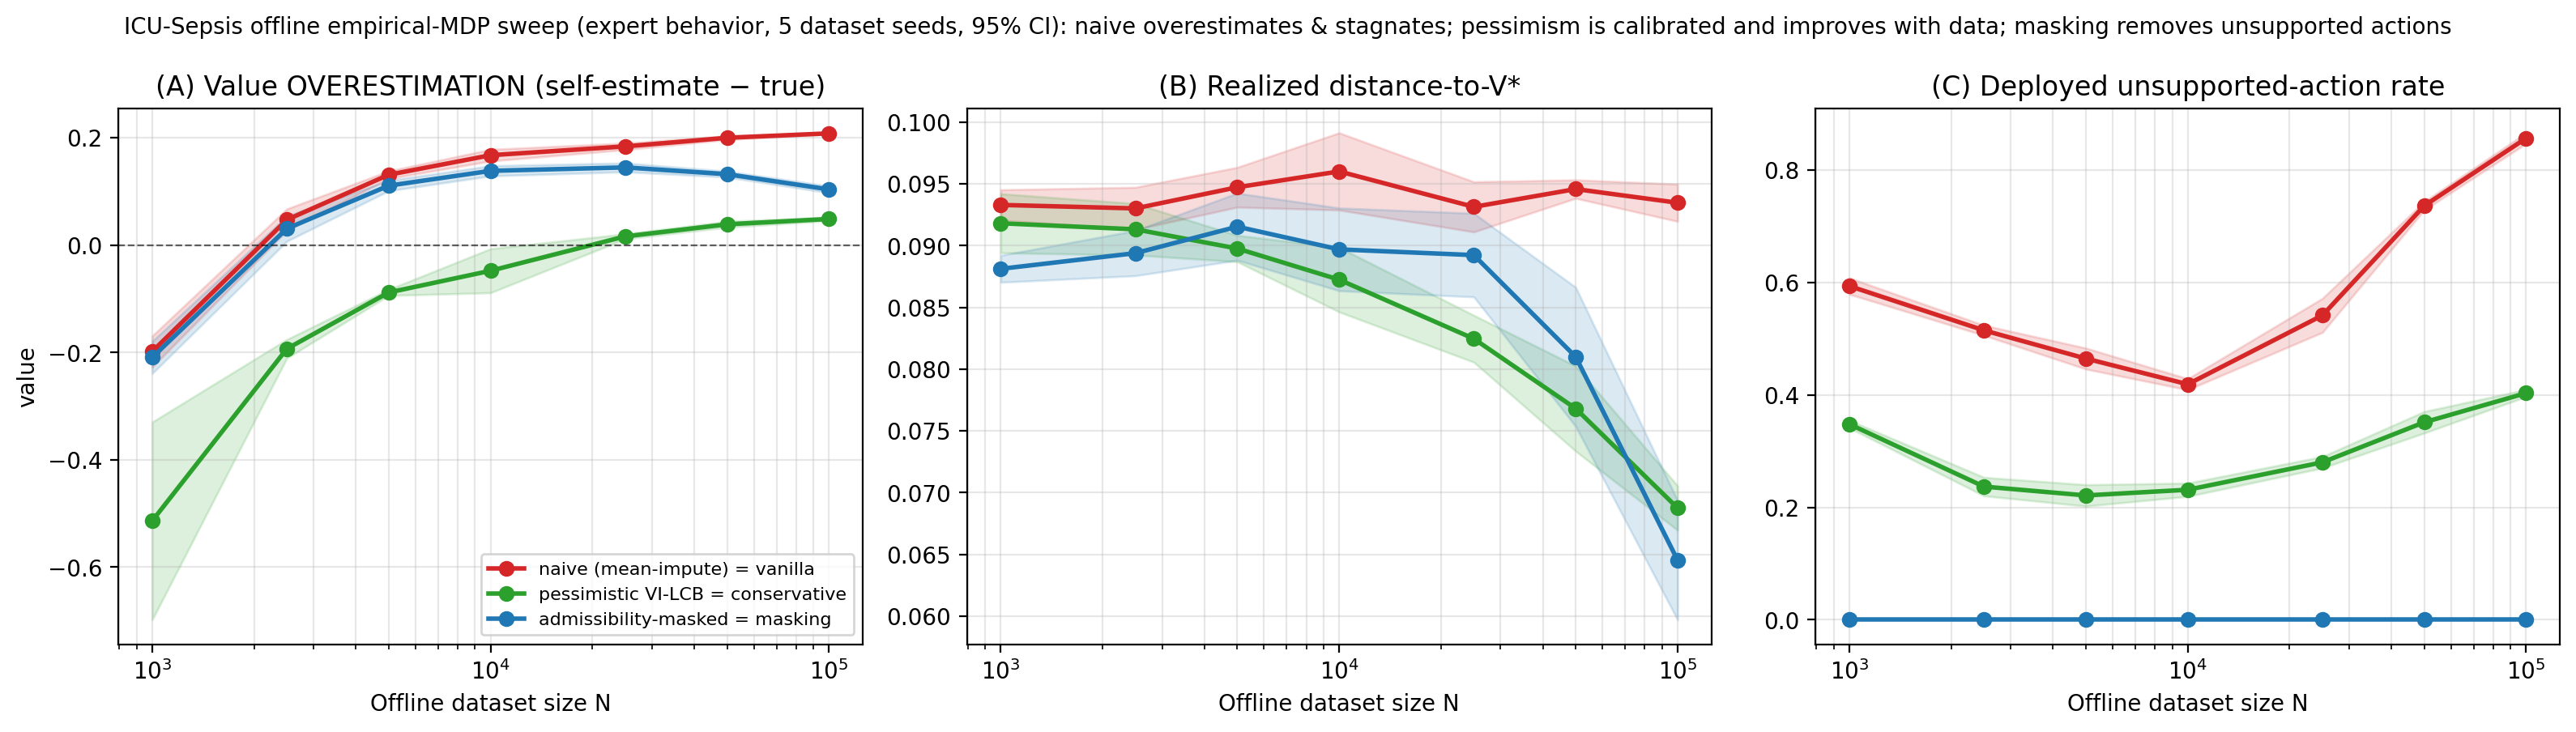
\includegraphics[width=0.95\linewidth]{offline_datasize.png}
\caption{Offline empirical-MDP sweep: naive mean-imputation overestimates its own
value and stagnates, while pessimism and masking are calibrated and improve with
data (5 seeds; exact evaluation against $V^\star$).}
\label{fig:offline}
\end{figure}

\subsection{Supplementary analyses}
\label{sec:supp}
We summarize defenses and robustness checks; figures are in the appendix.
\textbf{Expert projection (App.~\ref{app:figs}).} The benchmark's estimated, stochastic clinician policy places $\sim$16\% of its
per-state probability mass (averaged over non-terminal states) on inadmissible
actions---i.e.\ actions below the $\tau{=}20$ support threshold (low data support,
not never taken or medically invalid); clinician-guided exploration leaves $8\%$
deployed unsupported, but \emph{projecting} the prior onto $\Adm(s)$ drives this to
$0.5\%$ while preserving value and raising clinician agreement to $0.65$ --- support
projection, not imitation learning.
\textbf{Robustness (App.~\ref{app:figs}).} The failure and its fix hold across
Q-learning, SARSA, and Dyna-Q; under the \texttt{terminate} strategy (inadmissible
$\to$ death) vanilla agents naturally avoid unsupported actions (deploy
$85\%{\to}3$--$4\%$), confirming the failure is specific to \texttt{mean} --- though
model-free $\dist$ then \emph{worsens} ($0.107$/$0.108$ for Q/SARSA), and masking
remains best and most stable under either strategy.
\textbf{No dead-ends (App.~\ref{app:figs}).} Motivated by clinical dead-end analysis
\citep{fatemi2021deadends}, we find ICU-Sepsis has \emph{none}
($\min_s V^\star(s){=}0.198$; 427/713 states ``secured'' with $V^\star{>}0.9$);
mean imputation also compresses the higher one-step death risk of inadmissible
actions ($0.032$ vs.\ $0.023$) --- an honest negative result that supports the main
line.
\textbf{Severity and clinician composition.} Under exact evaluation, adding SOFA
shaping or a KL-to-clinician term on top of AA-MBRL (or AA-PPO) leaves the value
essentially unchanged (the AA-MBRL family all within $\sim$$0.0003$ of $J{=}0.874$,
the AA-PPO family within $\sim$$0.0007$ of $0.869$): the small per-prior gains and KL
variance-reduction reported under the benchmark's rollout metric do not survive exact
evaluation.\footnote{Composition policies are from the teammate runs, exact-evaluated;
masking does converge faster on the rollout learning curves ($\sim$1.8$\times$).}

% =============================================================================
\section{Discussion}
\label{sec:discussion}
\paragraph{Why survival rate hides the failure.}
Survival values occupy a narrow band ($0.78$--$0.875$) and the benchmark's headline
metrics (return, length, convergence) are insensitive to \emph{which} action is
chosen when inadmissible actions behave like random admissible ones. Detecting the
pathology therefore requires multi-metric, exact-$V^\star$ evaluation
(selection rate, $\dist$, $Q$-leakage), not survival rate alone.

\paragraph{Why a known-dynamics benchmark.}
Exact $V^\star$ is a \emph{measurement instrument}, not an optimization claim. The
OOD-action pathology---and the value overestimation it induces---is a general and well-recognized property of offline
RL \citep{kumar2020cql,kumar2019bear}; ICU-Sepsis simply lets us measure it cleanly,
sidestepping the noisy off-policy estimation that real cohorts force
\citep{gottesman2019guidelines}. We make no claim that the benchmark is more
realistic than real data---only that it is a particularly clean ruler.

\paragraph{Difference from the benchmark's own perturbation check.}
ICU-Sepsis includes a perturbation analysis (Appendix~B.3 of
\citealp{choudhary2024icusepsis}) that measures \emph{return robustness} and finds
the environment insensitive---which is expected by construction, since mean
imputation makes inadmissible actions return-equivalent to random admissible ones.
We instead measure selection rate, $\dist$, the learning mechanism, and a remedy
spectrum, which is where the cost actually shows up.

\paragraph{Benchmark guidance.}
ICU-Sepsis results should report inadmissible-action handling explicitly
(the strategy used, the deployed-unsupported rate, and $\dist$), rather than leaving
it to a hidden default. We release one-command scripts implementing the three
exactly-computable diagnostics.

\paragraph{What transfers, and what does not.}
Our constructive results---that admissibility masking and an
admissibility-constrained empirical model recover near-optimal value---are
\emph{benchmark-internal} and do not imply that a deployable offline medical-RL
system can ``close the gap.'' Three properties bound this. First, an optimality gap
is definable only because the benchmark treats its estimated model as ground truth
and exposes an exact $V^\star$; in a real cohort $V^\star$ is unknown and the gap is
unmeasurable, leaving only noisy, biased off-policy estimation
\citep{gottesman2019guidelines}. Second, the model-based remedy that reaches
$V^\star$ re-solves the very $716$-state model \emph{online}, which is inapplicable
offline and unsurprising at this scale \citep{auer2008ucrl,osband2013psrl}. Third,
the per-state priors are not external gifts but statistics of the same logged cohort,
so ``using the structure'' means computing support, a behavior policy, and severity
from one's own data. What transfers is thus not the score but the
\emph{support-aware principle}---treat data-unsupported actions with explicit
pessimism rather than imputing them to an average \citep{fujimoto2019bcq,kumar2020cql},
reinforced by our finite-data study (\S\ref{sec:offline})---together with the
exact-$V^\star$ auditing protocol; the gap-closing numbers remain a property of the
benchmark.

\paragraph{Significance for offline medical RL.}
Offline medical RL inherently learns from logged data with uneven action coverage,
and how a pipeline handles data-unsupported actions is a consequential design choice
that survival rate can hide. Our contribution is to make this failure visible and
exactly measurable on a controlled testbed, localize its mechanism, and package a
support-aware diagnostic-and-remedy protocol---a methodological caution and
evaluation protocol, not a clinical recommendation.

% =============================================================================
\section{Limitations}
\label{sec:limitations}
Our study is benchmark-internal and tabular: ``unsupported'' means insufficient data
support, not medical incorrectness, and we make no clinical claims. Whether the
mean-imputation failure and the behavior-masking fix transfer to function-approximation
/ continuous / deep settings is untested; in particular we do not evaluate SAC or
genuinely deep/continuous agents, and the offline empirical-MDP sweep is a step
toward the realistic finite-data regime but remains tabular. We use 5 seeds (effect
sizes for the support diagnostics are large, e.g.\ 87\%$\to$0\% deployed unsupported
and leakage $+0.46\to-0.80$). The clinician policy itself is not fully
admissibility-respecting, a property of the benchmark we inherit.

% =============================================================================
\section{Conclusion}
\label{sec:conclusion}
ICU-Sepsis's default mean-imputation makes data-unsupported actions look average, so
model-free agents adopt them at a value cost that survival rate hides. Using the
benchmark's exact $V^\star$, we localize the failure to behavior-level sampling,
explain it through an exact $Q$-value-leakage diagnostic, and compare support-aware
remedies online, across algorithms, and offline. Inadmissible-action handling should
be reported, not left to a hidden default: the gap was an artifact of mean-imputation,
and the environment ships the cure.

% =============================================================================
\section*{Reproducibility statement}
All mechanism experiments (baselines, component ablation, penalty sweep, offline
data-size sweep, expert projection, robustness, dead-end analysis) are computed from
the shipped ICU-Sepsis dynamics with exact value iteration and are reproducible from
the released one-command scripts; metric definitions are given in \S\ref{sec:method}.
Cross-algorithm and model-based ($5{\times}10^5$-episode) results are obtained by
\emph{exactly} evaluating the teammate's saved policies (committed in the released
repo) against the true dynamics; the evaluation script is released with our code, so
every number in Table~\ref{tab:merged} is reproducible.

% =============================================================================
\bibliographystyle{plainnat}
\bibliography{references}

% =============================================================================
\appendix
\section{Supplementary figures}
\label{app:figs}
This appendix collects the figures for the supplementary analyses discussed in
\S\ref{sec:supp} (expert projection, robustness across algorithms and strategies,
and dead-end structure).

\begin{figure}[t]\centering
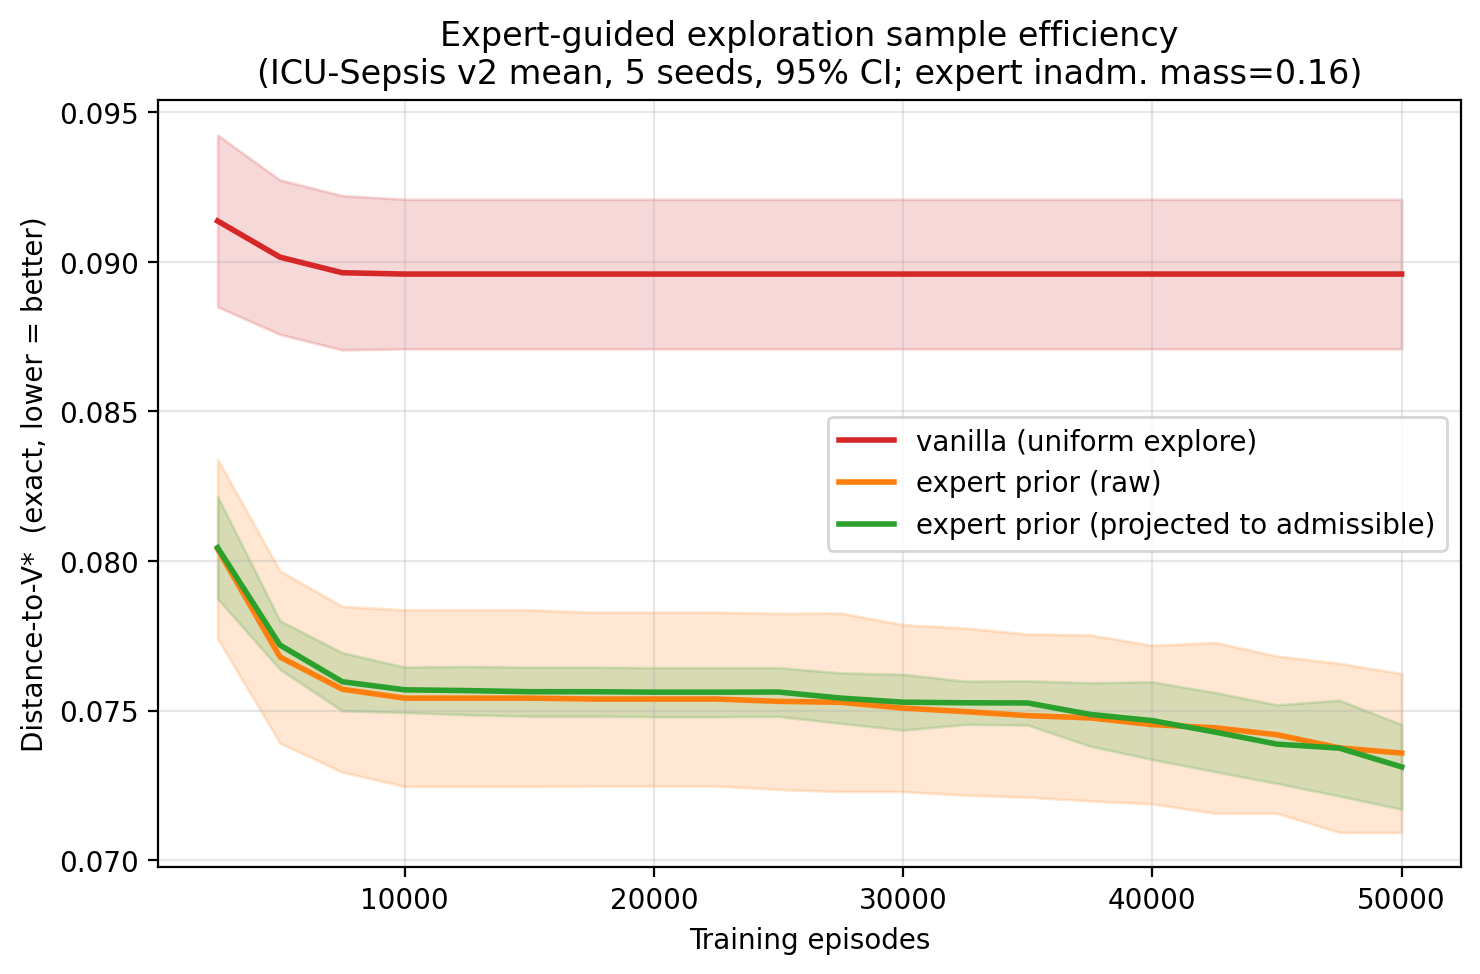
\includegraphics[width=0.6\linewidth]{expert_prior_curve.png}
\caption{Expert-guided exploration; admissible projection drives deployed
unsupported actions to $0.5\%$ while preserving value (5 seeds, $5{\times}10^4$
episodes).}
\label{fig:expert}
\end{figure}

\begin{figure}[t]\centering
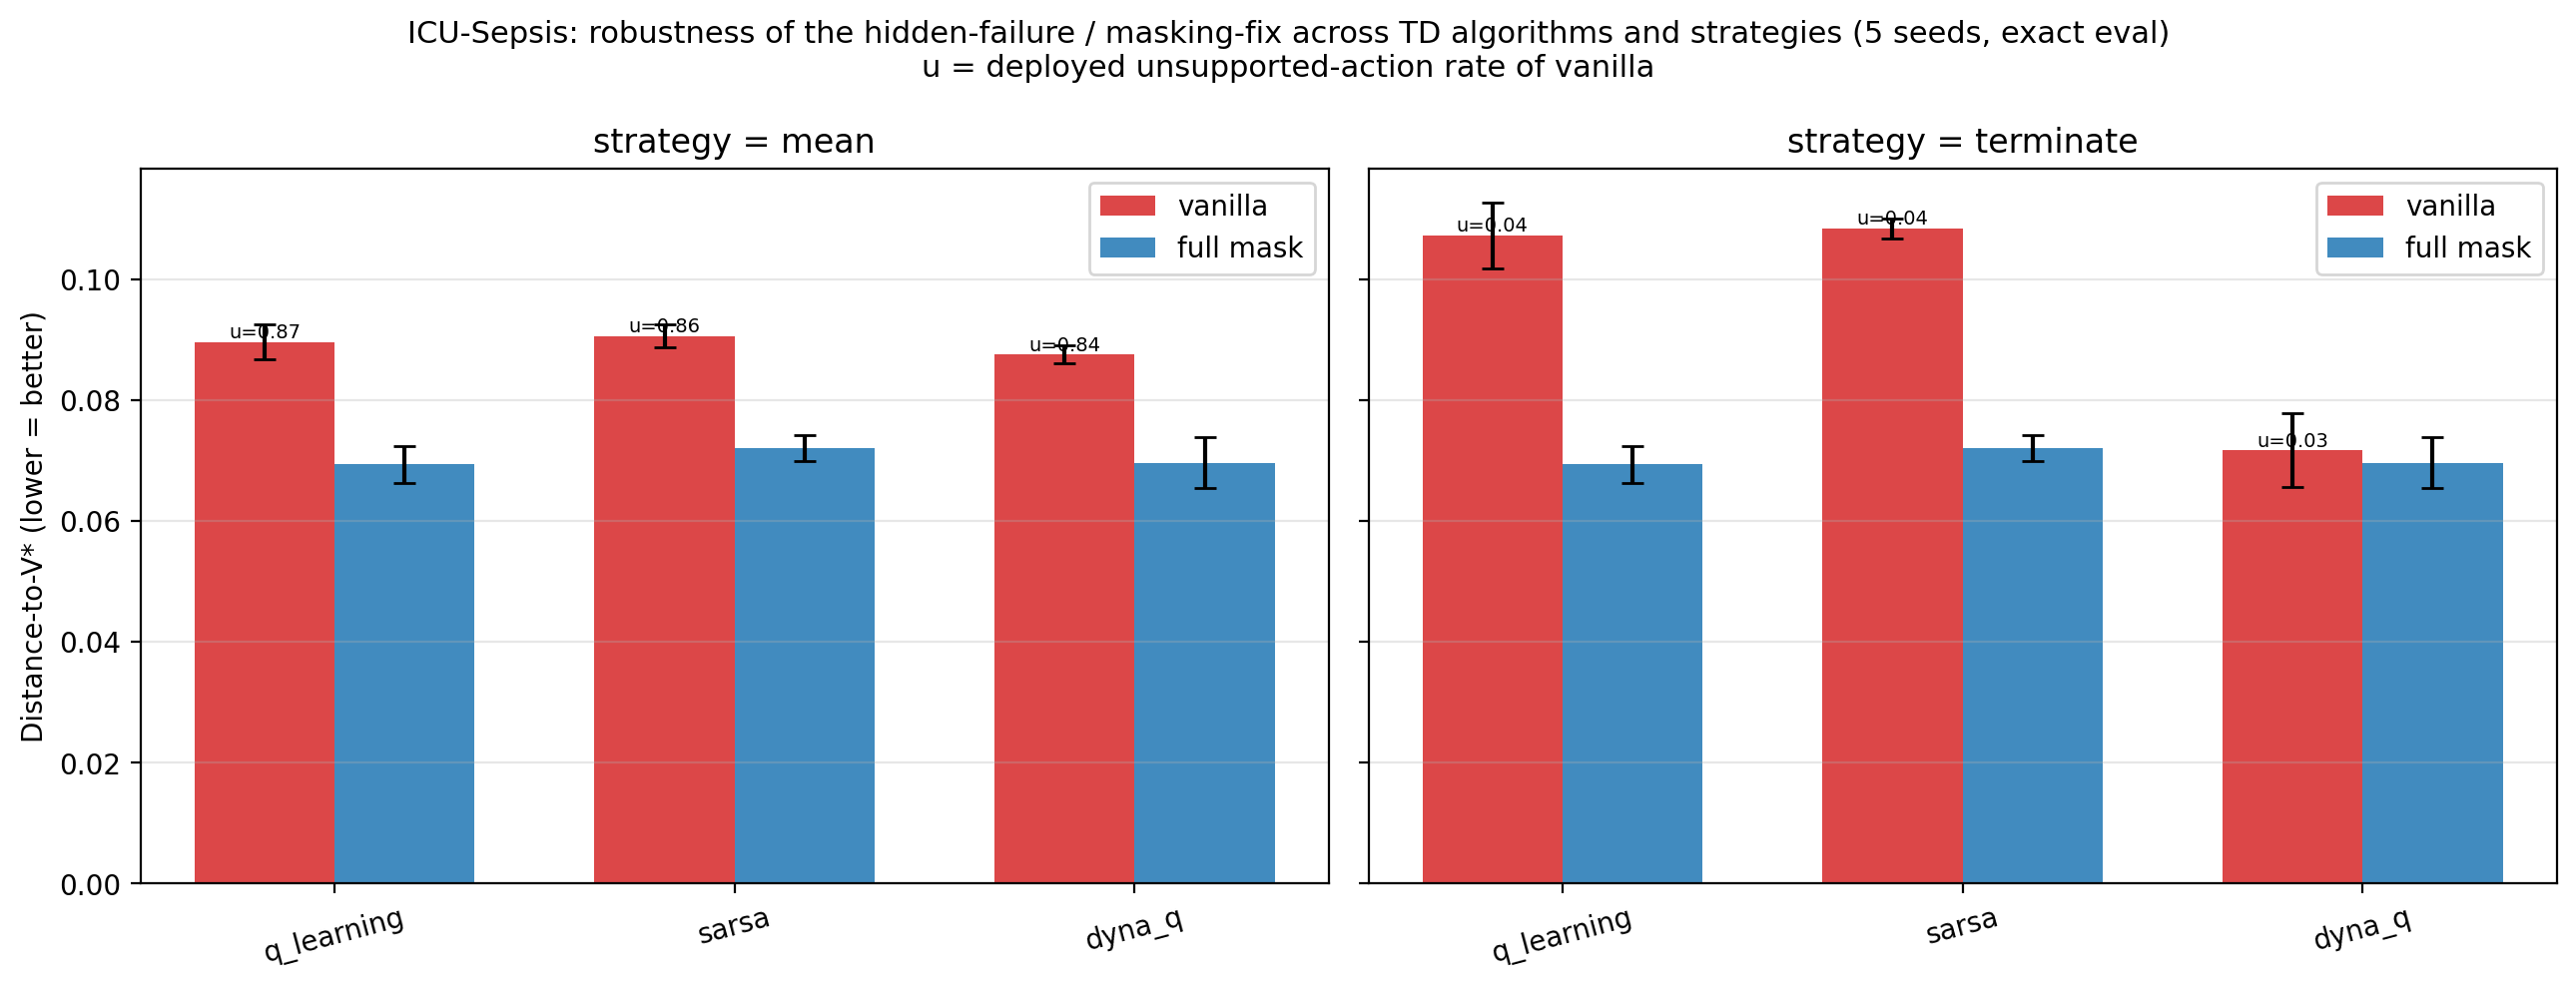
\includegraphics[width=0.95\linewidth]{robustness.png}
\caption{Robustness across algorithms (Q/SARSA/Dyna-Q) and imputation strategies
(\texttt{mean}/\texttt{terminate}); masking is best and most stable throughout
(5 seeds, $5{\times}10^4$ episodes).}
\label{fig:robust}
\end{figure}

\begin{figure}[t]\centering
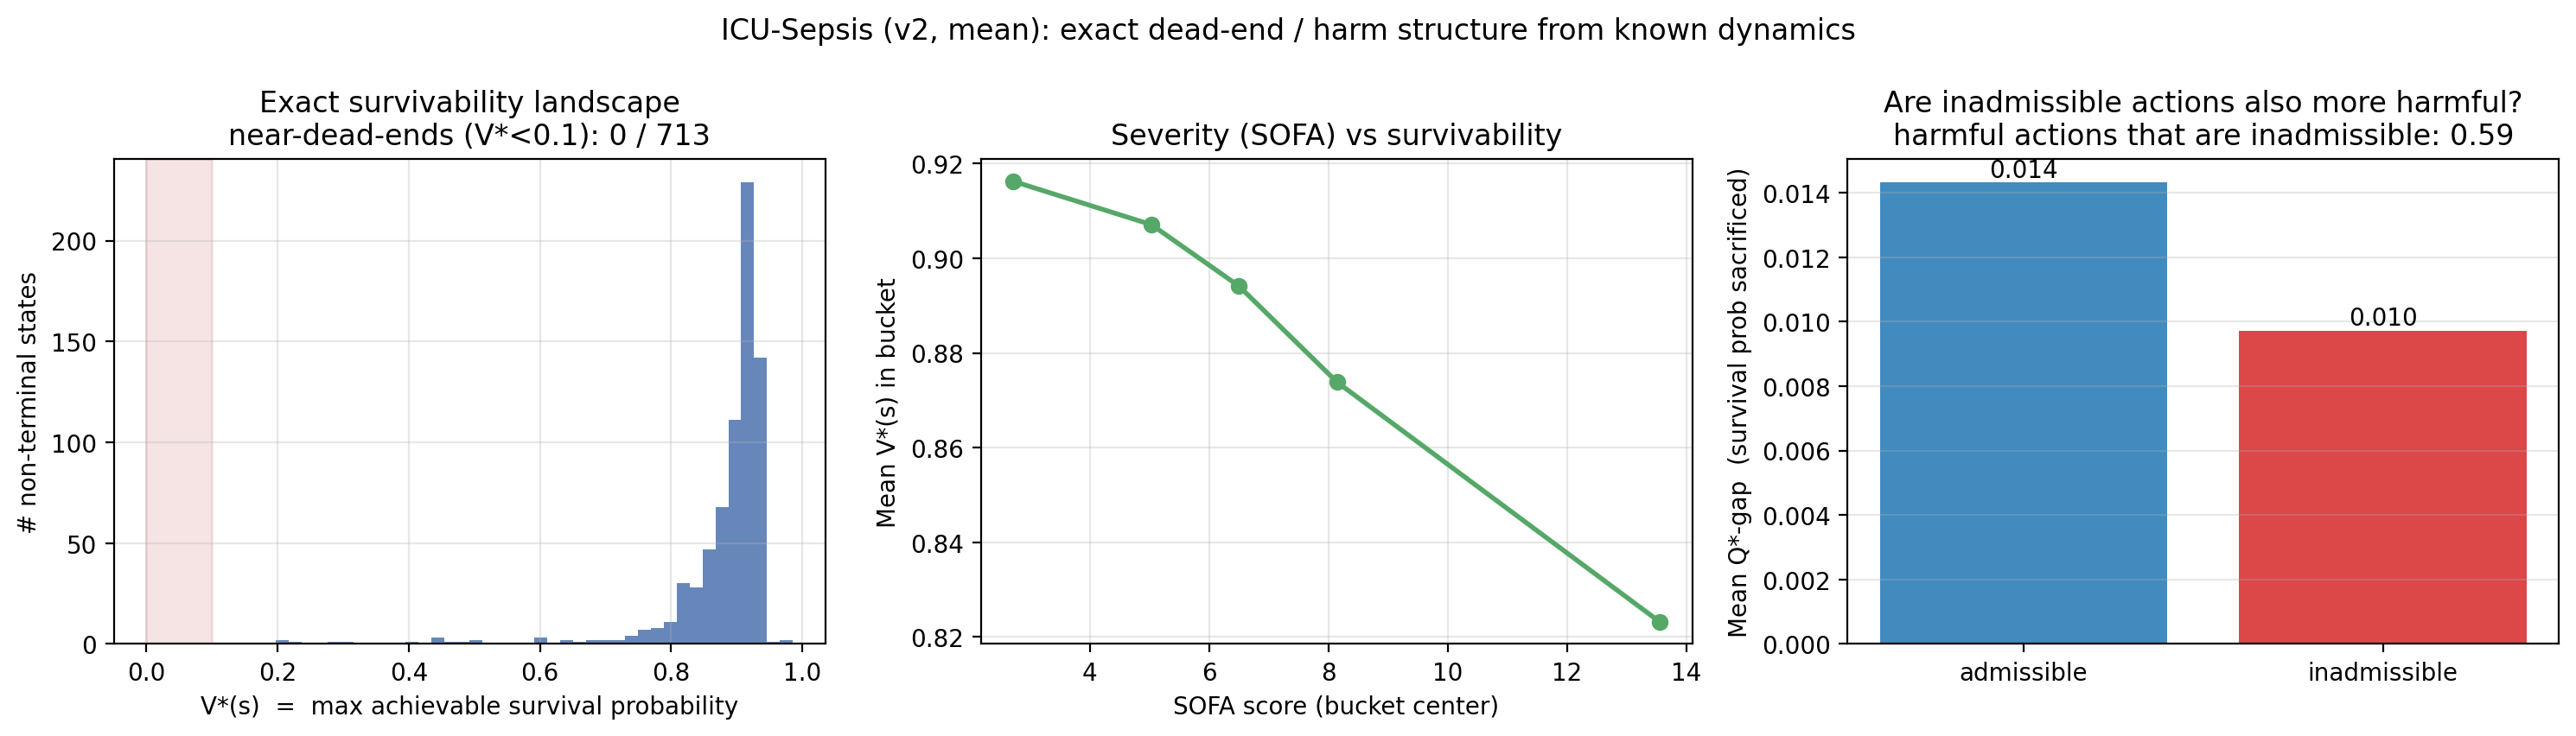
\includegraphics[width=0.95\linewidth]{deadend_structure.png}
\caption{Dead-end analysis: ICU-Sepsis has no dead-ends ($\min_s V^\star(s){=}0.198$;
427/713 states secured with $V^\star{>}0.9$).}
\label{fig:deadend}
\end{figure}

\end{document}
